\chapter{Index Analysis of the Modified Nodal Analysis}
\label{sec:index analysis of the modified nodal analysis}

%seite 22 kap 7 netw top and dae ind for rlc - modelling and discretization circ prob

In the previous chapter we have seen two different kinds of index concepts for differential algebraic equations. We have also seen that these two, even though they describe rather different structural aspects of the equation, are identical for the problems discussed in this thesis. %(i.e. linear?)
This leads to the question, what indices we expect to obtain for our MNA system.

This chapter answers this question for the case of linear RLC-circuits. It builds upon results discussed in \cite{ModellingAndDiscretizationOfCircuitProblems}, \cite{NumerikGewöhnlicherDifferentialgleichungen} and \cite{shashkov_tuprints27452}.
As already discussed in Section \ref{Sec:Components relations}, RLC circuits contain only resistors, inductors and capacities as well as current and voltage sources. Linear means that all circuit components are described by linear positive functions. Thus the matrices $C$, $R$, and $L$ are positive definite and symmetric.

Recall that we consider the equations resulting from the analysis in Section \ref{sec:MNA}. These equations are of the form \eqref{DAE-const-coeff}: Find $y$ such that
\begin{displaymath}
	A y'(t) + B y(t) = f(t).
\end{displaymath}
In particular we obtain the system of equations
\begin{displaymath}
	\begin{pmatrix}
		A_C C A_C^\top & 0 & 0 \\
		0 & L & 0 \\
		0 & 0 & 0
	\end{pmatrix}
	*
	\begin{pmatrix}
		u' \\
		i_L' \\
		i_V'
	\end{pmatrix}
	+
	\begin{pmatrix}
		A_R G A_R^\top & A_L & A_V \\
		-A_L^\top & 0 & 0 \\
		-A_V^\top & 0 & 0 ä
	\end{pmatrix}
	*
	\begin{pmatrix}
		u \\
		i_L \\
		i_V
	\end{pmatrix}
	=
	\begin{pmatrix}
		-A_I i_{src} \\
		0 \\
		-v_{src}
	\end{pmatrix}.
\end{displaymath}

\section{General Index analysis}

Assuming the system only contains linear elements, then the corresponding network equation represents a DAE with constant coefficients \eqref{DAE-const-coeff}. We collect all unknowns in $y(t)=(u(t), i_L(t), i_V(t))^\top$. The structure of the system is reliant on the matrix $B$, thus we consider two cases.

\paragraph{ODE-case:}
	The matrix $B$ in \eqref{DAE-const-coeff} is regular. This is the case iff the circuit contains no voltage sources and every node has a path to ground, that leads through at least one capacitor. Then the system represents a linear-implicit system of ODEs and can be transformed into the explicit ODE sytstem
	\begin{displaymath}
		y(t)'=B^{-1}(-Ay(t)+f(t)).
	\end{displaymath}
	Thus we obtain an index of $0$.
		
\paragraph{DAE-case:}
	The matrix $B$  in \eqref{DAE-const-coeff} is singular. This is the interesting case which we will analyse in the following.


For a singular matrix $B$ we have already obtained a representation of the form
\begin{align*}
	u'(t) + Ru(t) &= s(t), \\
	Nv'(t) + v(t) &= q(t)
\end{align*}
in the previous section, see \eqref{transformed-DAE-const-coeff}. We now consider the nilpotency index $\nu$ of the matrix $N$, since we already know that this index correlates with the differentiation index as well as the perturbation index. We consider two cases:

\begin{enumerate}
	\item \textbf{The nilpotency index is 1} \newline
		Because $N$ is nilpotent with nipotency index $\nu = 1$, it holds that $N^1 = 0$, thus the system transforms to
		\begin{align*}
			u'(t) + Ru(t) &= s(t), \\
			v(t) &= q(t).
		\end{align*}
		This means that the algebraic variables are given explicitly. Thus the system is in ODE form.

	\item \textbf{The nilpotency index is $\geq$ 2} \newline
		This case is the situation we have discussed in section \ref{chap:Weierstraß-Kronecker Normalform}, where we obtained the representation \eqref{solution-to-transformed-DAE-const-coeff-part2}
		\begin{equation}
			\label{eq:representation differential variable with nilpotency index}
			v(t) = \sum_{i=0}^{\nu-1} (-1)^iN^iq^{(i)}(t).
		\end{equation}
		By differentiating the above equation one more time, we obtain
		\begin{equation}
			\label{eq:hidden constraint}
			v'(t) = \sum_{i=0}^{\nu-1} (-1)^iN^iq^{(i+1)}(t)
		\end{equation}
		with the assumption that $q$ is $\nu$ times differentiable.
\end{enumerate}

We observe that in both cases the solution $v$ has to fulfill an algebraic constraint. In the case of index $\nu = 1$ this equation is given explicitly, while for index $\nu \geq 2$ it is given implicitly by \eqref{eq:hidden constraint}.

This system is also sensitive to perturbations. Note that the solution formula \eqref{eq:representation differential variable with nilpotency index} for $v$ also contains derivatives of the input $q$. Thus small noise in the input can have arbitrarily large derivatives, which can influence the solution.

%This means no severe numerical problems arise from index-1 systems. Implicit numerical integration schemes for stiff systems are feasable. On the other hand severe nunmerical problems may occur in the case that the system has index greater or equal to $2$. The hidden constraints can only be resolved by an unstable differentiation process.

%As the Kronecker index $k=ind\{A,B\}$ defines the behaviour of the system theoretically as well as numerically it is called the \emph{algebraic index} of the linear implicit system.

\section{Topological Conditions} 
%\cite{Tischendorf2005Topological}, %chapter 7 of
%\cite{ModellingAndDiscretizationOfCircuitProblems}
%\cite{DesoerCharlesA1969Bct}
%
%From analysing the MNA some conditions to the circuit topology can be obtained. We will be considering the impact of special arrangements of components on the index of the system. In \cite{Tischendorf2005Topological} they present results about the index of MNA equations.
%
%
%\begin{theorem}[Index-1 condition \cite{Tischendorf2005Topological}] \label{Index-1 condition}
%	Let the matrices of the capacitances, inductances and resistances be positive definite. If the network neither cointains \emph{inductance-current-source cutsets} nor (controlled?) \emph{capacitance-voltage-source loops}, then the MNA leads to an index-1 DAE.
%\end{theorem}
%
%Where inductance-current-source cutsets and capacitance-voltage-source loops are subcircuits of the form (Seite 481 (searchbar) in basic circuit theory)
%
%\begin{figure}[H]
%	\begin{subfigure}{0.5\textwidth}
%		\centering
%		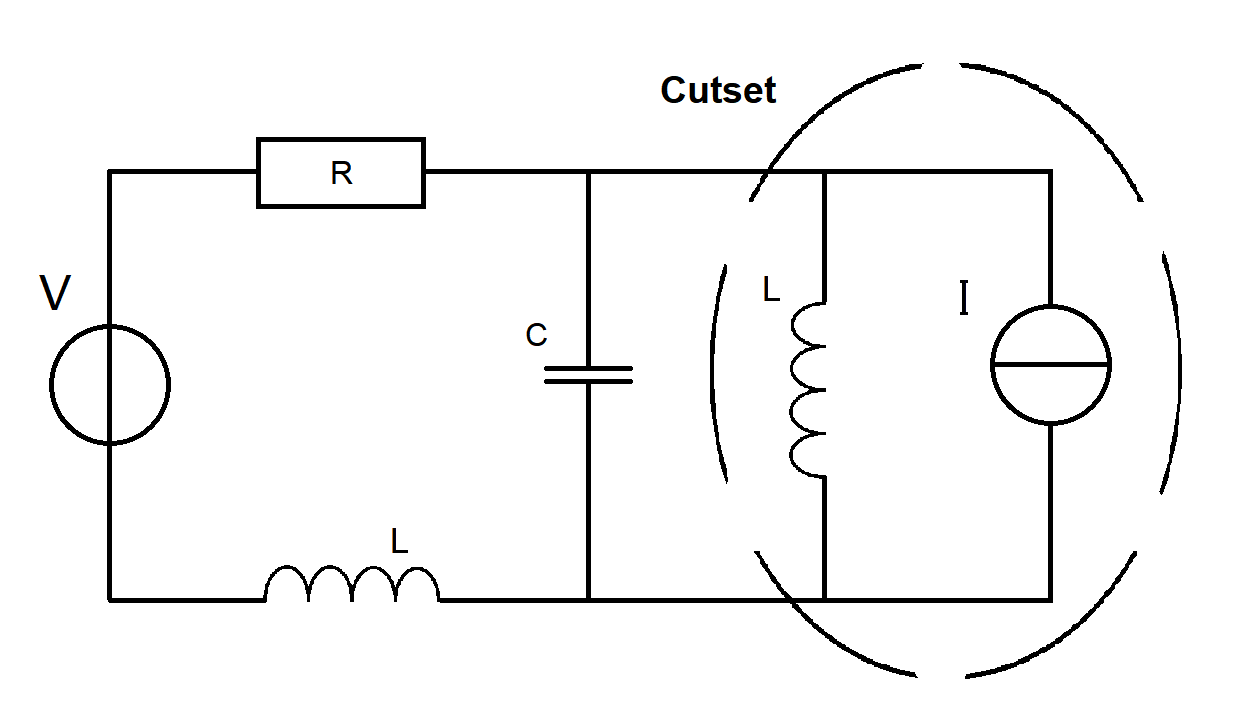
\includegraphics[width=0.9\linewidth]{pictures/inductance-current-source_cutset.png}
%		\caption{inductance-current-source cutset}
%	\end{subfigure}
%	\begin{subfigure}{0.5\textwidth}
%		\centering
%		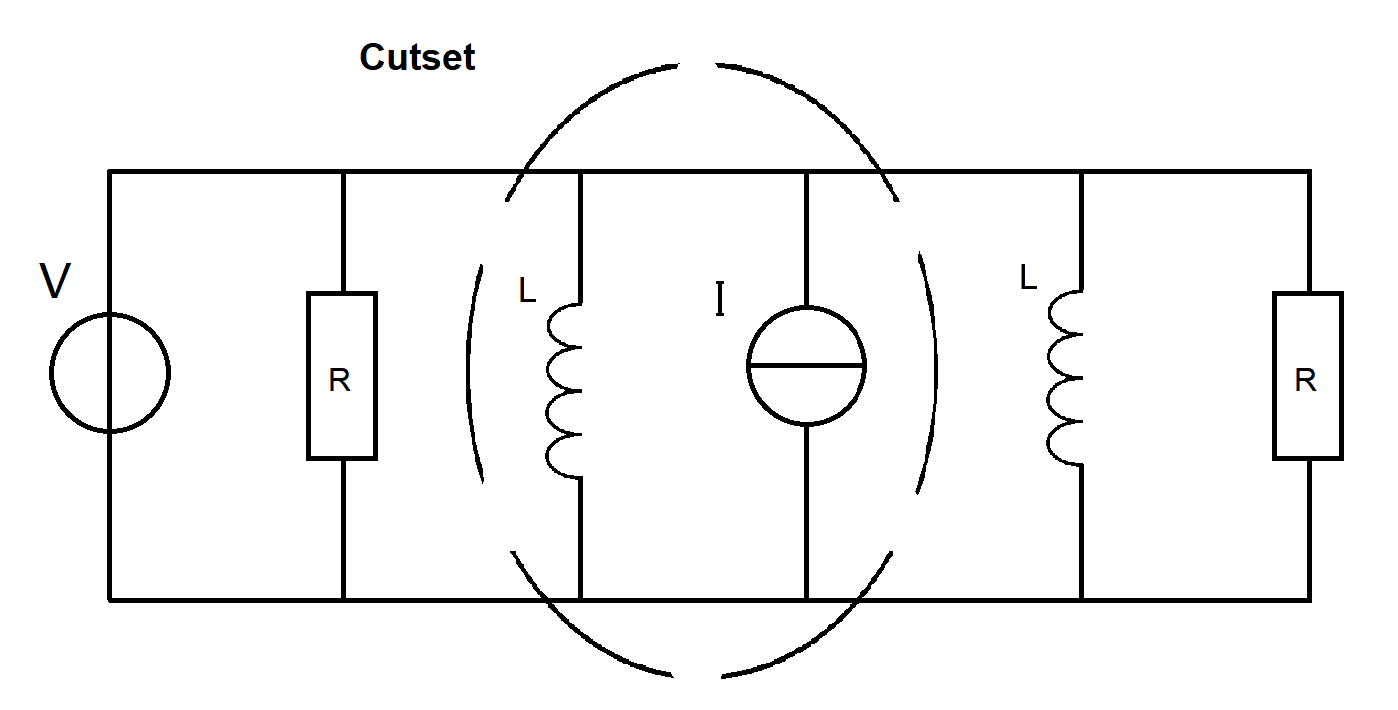
\includegraphics[width=0.9\linewidth]{pictures/capacitance-voltage-source_loop.png}
%		\caption{capacitance-voltage-source loop}
%	\end{subfigure}
%	\label{cutset and loop}
%	\caption{cutset and loop}
%\end{figure}
%
%This means that if our circuit does not contain any loops or cutsets of the above form the resulting MNA system has index 1.
%
%\begin{theorem}[Index-2 condition \cite{Tischendorf2005Topological}] \label{Index-2 condition}
%	If the Network contains \emph{inductance-current-source cutsets} or \emph{capacitance-voltage-source loops} except for capacitance-only loops, then the MNA leads to an index-2 DAE.
%\end{theorem}
%
%These results can also be interpreted in a more formal way. As they are just descriptions of the topology of the circuit we can reformulate the theorems in terms of the incidence matrix $A$.
%
%By perturbing the right hand side of of \eqref{MNA_Matrixform} with a slight perturbation $\delta = (\delta_C, \delta_L, \delta_V)^\top$ we get a corresponding solution $x^\delta = (u^\delta, i_l^\delta, i_V^\delta)^\top$. One can show that the difference of this perturbed solution to the solution $x$ of the unperturbed system is bounded by
%\begin{displaymath}
%	|| x^\delta - x(t) || \leq C * \left( ||x^\delta (0) - x(0)|| + \max_{0 \leq \tau \leq t} ||\delta(\tau)|| + \max_{0 \leq \tau \leq t} ||Q_{CRV}^\top \delta_C'|| + \max_{0 \leq \tau \leq t} ||\tilde{Q}_{V-C}^\top \delta_V'|| \right)
%\end{displaymath}
%
%using orthogonal projectors$Q_C$, $Q_{CRV}$ and $\tilde{Q}_{V-C}$  onto $ker(A_C^\top)$, $ker(A_CA_RA_V)^\top$ and $ker(Q_C^\top A_V)$ respectively. We denot $ker(A) = \{x: Ax = 0\}$.
%
%Hence, Theorem \ref{Index-1 condition} can be interpreted as the two conditions
%
%\begin{equation}
%	\label{eq:alt-condditions}
%	\begin{aligned}
%		kerQ_C^\top A_v &= {0}, \\
%		ker(A_C A_R A_V)^\top &= {0}.
%	\end{aligned}
%\end{equation}
%	
%
%This means that for ``reasonable'' RLC circuits, i.e. circuits satisfying the prerequisites of the above Theorem \ref{Index-1 condition}, the index will not exceed 2. We will only consider such circuits in this thesis.
%
%If one of the conditions \eqref{eq:alt-condditions} is violated, we are in the case of Theorem \ref{Index-2 condition} and thus have index 2.

%alternative version:

From analysing the MNA equations, some conditions to the circuit topology can be obtained. We will be considering the impact of special arrangements of components on the index of the system. General results are presented in \cite{Tischendorf2005Topological} as well as in \cite{shashkov_tuprints27452} and \cite{Reis2014}.


%theorem 6.14 aus large scale networks auch ähnlich

%%%%%%%%%%%%%%%%%%%%%%%%%%%%%%%%%%%%%%%%%%%%%%%%%%%%%%%%%%%%%%%pagebreak%%%%%%%%%%%%%%%%%%%%%%%%%%%%%%%%%%%%%%%%%%%%%%%%%%%%%%%%%%%%%%%%%%%%%%%%%%%%%%%%
\newpage
%%%%%%%%%%%%%%%%%%%%%%%%%%%%%%%%%%%%%%%%%%%%%%%%%%%%%%%%%%%%%%%%%%%%%%%%%%%%%%%%%%%%%%%%%%%%%%%%%%%%%%%%%%%%%%%%%%%%%%%%%%%%%%%%%%%%%%%%%%%%%%%%%%%%%%%%

\begin{theorem}[Index conditions \protect{\cite[Theorem~2.2.1]{shashkov_tuprints27452}}]
	Let the matrices of the capacitances, inductances and resistances be positive definite.
	\begin{itemize}
		\item If
		\begin{equation}
			\label{eq:index condition leq 2}
			ker([A_R, A_C, A_V, A_L]^\top) = \{0\} \quad \text{and} \quad ker(A_V) = \{0\}
		\end{equation}
		holds, then the MNA \eqref{MNA_Matrixform} leads to a system with index $\nu \leq 2$.
		
		\item If additionally
		\begin{equation}
			\label{eq:index condition leq 1}
			ker([A_R, A_C, A_V]^\top) = \{0\} \quad \text{and} \quad ker([A_C, A_V]) = \{0\}
		\end{equation}
		holds, then the system is of index $\nu \leq 1$
		
		\item If further
		\begin{equation}
			\label{eq:index condition eq 0}
			ker(A_C^\top) = \{0\} \quad \text{and} \quad dim(v_{src}) = 0
		\end{equation}
		holds, then the system has index $\nu = 0$.
	\end{itemize}
\end{theorem}

By $ker(A)$ we denote the nullspace of the matrix $A$ and by $dim(y)$ the size of the vector $y$. As \eqref{eq:index condition leq 2} - \eqref{eq:index condition eq 0} are just conditions concerning the topology of the circuit they can also be interpreted as follows:

\begin{itemize}
	\item Condition \eqref{eq:index condition leq 2} means that the circuit neither contains loops of voltage sources nor cutsets of current sources.
	\item Condition \eqref{eq:index condition leq 1} means that the circuit contains neither loops of capacitors and/or voltage sources nor cutsets of inductors and/or current sources.
	\item Condition \eqref{eq:index condition eq 0} means that every node in the circuit is connected to the reference node (ground) through a path containing only capacitors.
\end{itemize}

A cutset of a circuit is a part (subcircuit) of the circuit that can be separated from the main circuit by only ``cutting'' edges containing no components, the cutset and the original circuit without the cutset both cannot have any open edges. A loop is a subcircuit, which can be constructed by removing edges and nodes from the main circuit until we are left with only one continuous ``loop'' of edges and nodes. Figure \ref{fig:cutset and loop} illustrates the two concepts.

\begin{figure}[H]
	\begin{subfigure}{0.5\textwidth}
			\centering
			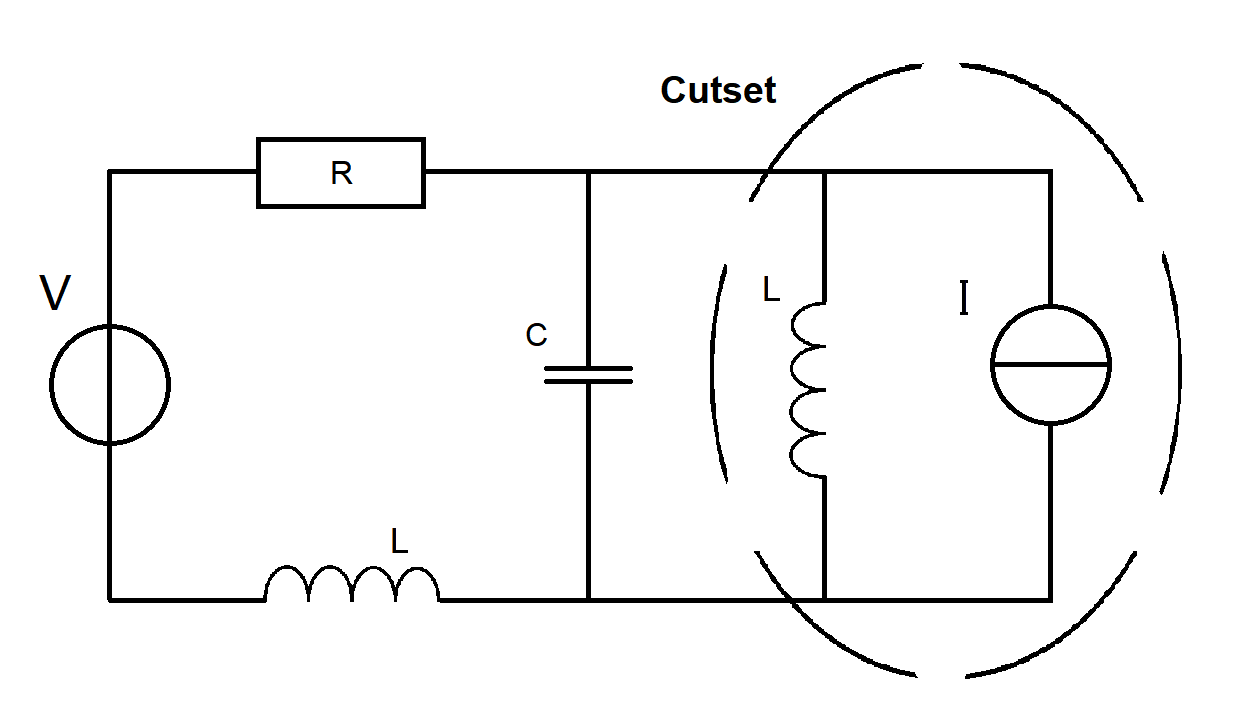
\includegraphics[height=4cm]{pictures/inductance-current-source_cutset.png}
			\caption{capacitor-voltage-source cutset}
		\end{subfigure}
	\begin{subfigure}{0.5\textwidth}
			\centering
			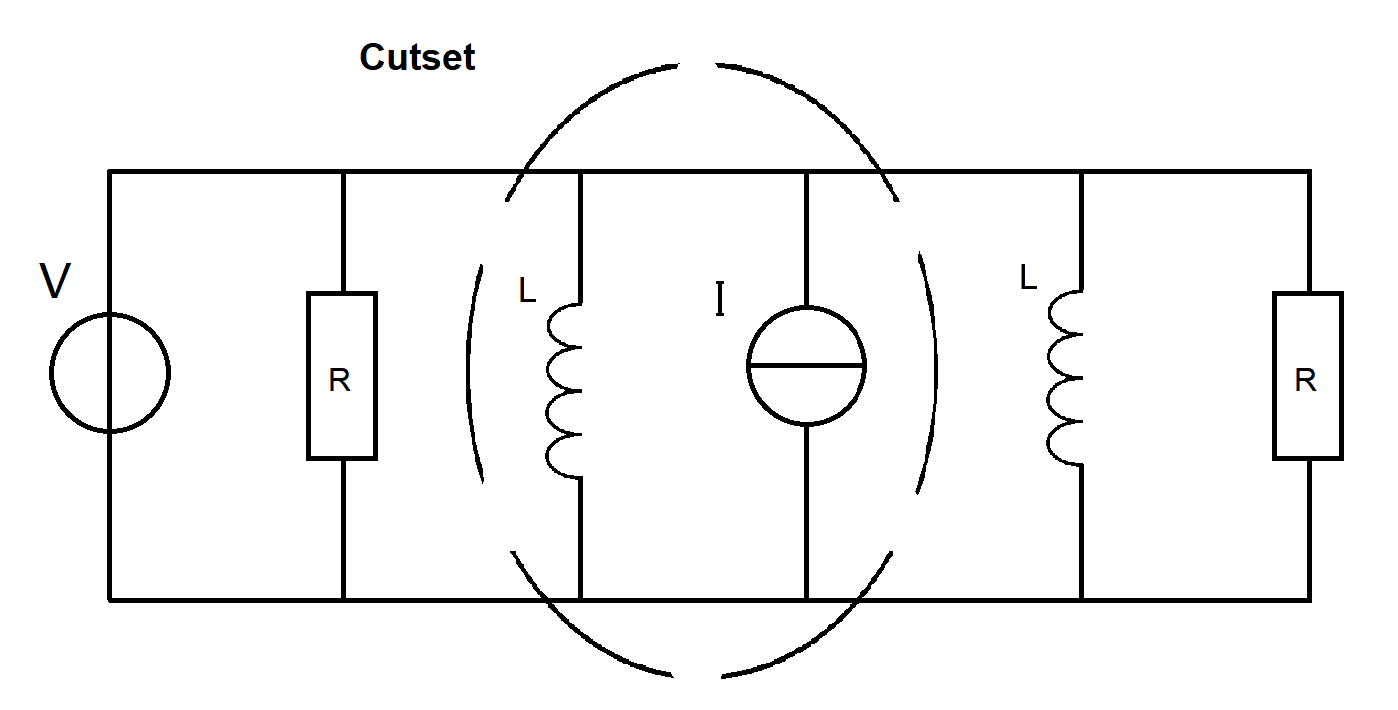
\includegraphics[height=4cm]{pictures/capacitance-voltage-source_loop.png}
			\caption{inductance-current-source loop}
		\end{subfigure}
	\caption{Illustration of a cutset and a loop.}
	\label{fig:cutset and loop}
\end{figure}

We will apply those results to the previously considered examples: 

\begin{example1}[Index analysis]
	\label{ex:Index_Analysis}
	As our first example we consider again the charging of a capacitor with a series resistor as in \textbf{Example 1}.
	\begin{figure}[H]
		\centering
		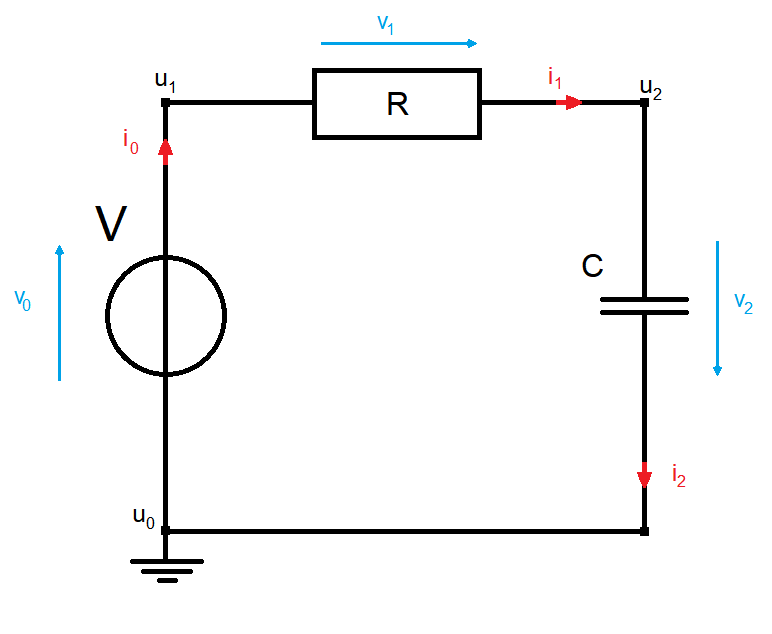
\includegraphics[scale = 0.4]{pictures/Example1_simple_p2.png}
		\caption{charging capacitor with series resistor and voltage source (note the difference to \ref{circuit:charging of capacitor})} 
	\end{figure}
	Because this circuit only contains one loop, which has a voltage source as well as a capacitor and a resistor we expect the resulting MNA system to be of index $\nu=1$. 
	
	The incidence matrix for this system is
	\begin{displaymath}
		A = [A_V, A_R, A_C] = 
		\left(
		\begin{matrix}
			-1 & 1 & 0 \\
			0 & -1 & 1 
		\end{matrix}
		\right).
	\end{displaymath} 
	Thus condition \eqref{eq:index condition leq 2} gives us
	\begin{displaymath}
		ker([A_R, A_C, A_V, A_L]^\top) = ker
		\left(
		\begin{matrix}
			1 & -1 \\
			0 & 1 \\
			-1 & 0
		\end{matrix}
		\right)
		= \{0\} 
		\quad \text{and} \quad 
		ker(A_V) = ker
		\left(
		\begin{matrix}
			-1 \\
			0
		\end{matrix}
		\right) = \{0\}.
	\end{displaymath}
	This condition is fulfilled, thus the index has to be smaller or equal to $2$.
	The condition \eqref{eq:index condition leq 1} results in
	\begin{displaymath}
		ker([A_R, A_C, A_V]^\top) = ker
		\left(
		\begin{matrix}
			1 & -1 \\
			0 & 1 \\
			-1 & 0
		\end{matrix}
		\right) 
		= \{0\} 
		\quad \text{and} \quad
		ker([A_C, A_V]) = ker
		\left(
		\begin{matrix}
			0 & -1\\
			1 & 0
		\end{matrix}
		\right) = \{0\}.
	\end{displaymath}
	Thus the index also has to be smaller or equal to $1$. 
	Finally condition \eqref{eq:index condition eq 0} results in
	\begin{displaymath}
		ker(A_C^\top) = ker
		\left(
		\begin{matrix}
			0 & 1
		\end{matrix}
		\right) 
		= \{0\} 
		\quad \text{and} \quad
		dim(v_{src}) \neq 0.
	\end{displaymath}
	This means that this system has index $\nu = 1$.
\end{example1}


	
\begin{example2}[Index analysis]
	This example depicts an energy conserving system. The electric energy stored in the capacitor is converted into the the magnetic energy of the coil and vice versa.
	\begin{figure}[H]
		\centering
		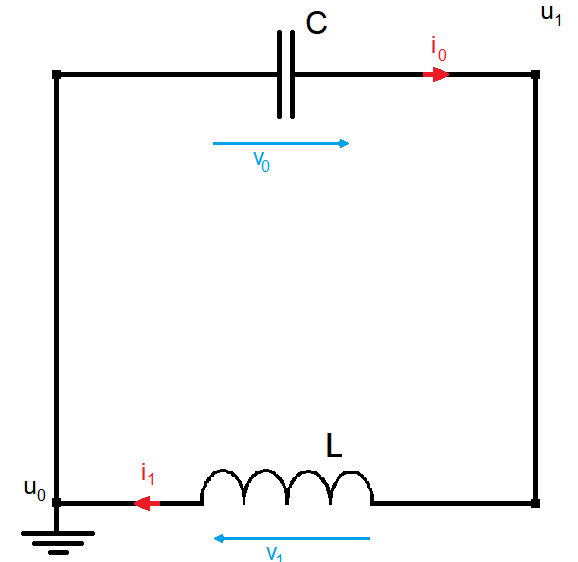
\includegraphics[scale = 0.4]{pictures/Example2_index0.png}
		\caption{LC circuit}
	\end{figure}
	Because this circuit only contains one capacitor and one inductance in a singular loop and also has no sources, we expect the resulting MNA system to be of index $\nu=0$. This means that the system is an ODE.
	
	The incidence matrix for this system is
	\begin{displaymath}
		A = [A_L~A_C] = 
		\left(
		\begin{matrix}
			-1 & 1
		\end{matrix}
		\right).
	\end{displaymath} 
	Thus condition \eqref{eq:index condition leq 2} gives us
	\begin{displaymath}
		ker([A_R, A_C, A_V, A_L]^\top) = ker
		\left(
		\begin{matrix}
			-1 \\
			1
		\end{matrix}
		\right) = \{0\}
		\quad \text{and} \quad 
		ker(A_V) = \{0\}.
	\end{displaymath}
	This condition is fulfilled, thus the index has to be smaller or equal to 2. \\
	Condition \eqref{eq:index condition leq 1} results in
	\begin{displaymath}
		ker([A_R, A_C, A_V]^\top) = ker\left(
		\begin{matrix}
			-1
		\end{matrix}
		\right) = \{0\}
		\quad \text{and} \quad
		ker([A_C, A_V]) = ker
		\left(
		\begin{matrix}
			-1
		\end{matrix}
		\right) = \{0\}.
	\end{displaymath}
	This condition is also fulfilled, thus the index has to be smaller or equal to 1.\\
	Finally condition \eqref{eq:index condition eq 0} results in
	\begin{displaymath}
		ker(A_C^\top) = ker\left(
		\begin{matrix}
			-1
		\end{matrix}
		\right) = \{0\}		
		\quad \text{and} \quad 
		dim(v_{src}) = 0.
	\end{displaymath}
	Thus it is fulfilled and we obtain index 0.
	
	If we have consider the MNA directly, we also see that this system is of index $\nu = 0$, because the MNA has the form
	\begin{displaymath}
		\begin{aligned}
			C u'_1 - i_L &= 0, \\
			L u'_L + u_1 &= 0
		\end{aligned}
	\end{displaymath}
	which is clearly a system of ODEs.
\end{example2}
	
\begin{example3}[Index analysis]
	Finally, as the third example seems very similar to the first one, we might also expect them to have the same index. But this is indeed not the case as the following analysis shows. 
	\begin{figure}[H]
		\centering
		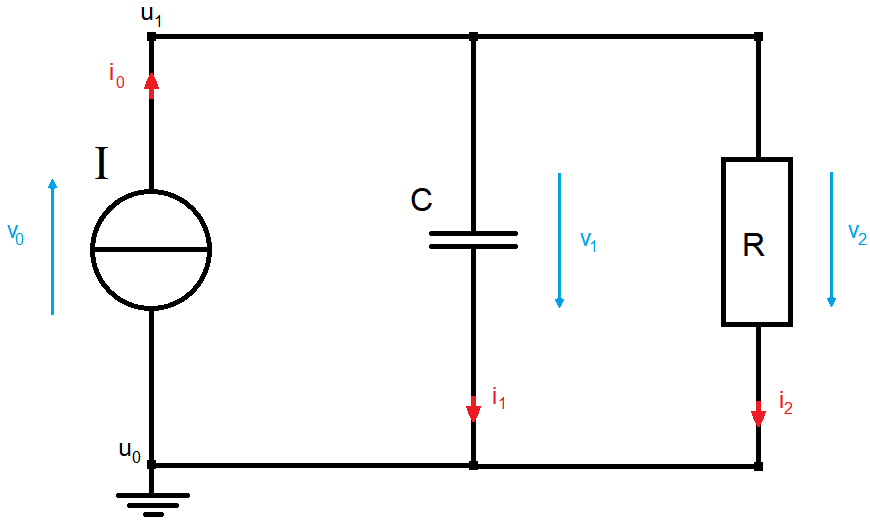
\includegraphics[scale = 0.4]{pictures/Example3.png}
		\caption{current source with resistor and capacitor} 
	\end{figure}
	This circuit contains two loops, the first with only a voltage source and a capacitor and the second with a capacitor and a resistor. Because of the first loop, we expect this circuit to emit a system of index $\nu = 2$.
	
	The incidence matrix for this system is
	\begin{displaymath}
		A = [A_V~A_C~A_R] = 
		\left(
		\begin{matrix}
			-1 & 1 & 1
		\end{matrix}
		\right).
	\end{displaymath} 
	Thus condition \eqref{eq:index condition leq 2} gives us
	\begin{displaymath}
		ker([A_R, A_C, A_V, A_L]^\top) = ker
		\left(
		\begin{matrix}
			1 \\
			1 \\ 
			-1
		\end{matrix}
		\right) = \{0\}
		\quad \text{and} \quad 
		ker(A_V) = ker
		\left(
		\begin{matrix}
			-1
		\end{matrix}
		\right) = \{0\}
	\end{displaymath}
	This condition is fulfilled, thus the index has to be smaller or equal to 2.
	Condition \eqref{eq:index condition leq 1} results in
	\begin{displaymath}
		ker([A_R, A_C, A_V]^\top) = ker\left(
		\begin{matrix}
			1 \\
			1 \\
			-1
		\end{matrix}
		\right) = \{0\}
		\quad \text{and} \quad
		ker([A_C, A_V]) = ker
		\left(
		\begin{matrix}
			1 & -1
		\end{matrix}
		\right) \neq \{0\}.
	\end{displaymath}
	Thus this condition is not fulfilled, which means that the system indeed has index $\nu = 2$.
\end{example3}
	
	
\section{Consistent Initial Values}
\label{sec:consistant initial values}

When solving a problem numerically, it is important to ensure that the problem has a (unique) solution. Without a solution, a numerical method could converge to an arbitrary value unrelated to any actual solution. In real-world applications, there may be multiple possible initial values. To guarantee a (unique) solution, it is crucial to choose initial values that are consistent. This is why identifying conditions for constructing \emph{consistent} initial values is important. For further details, see \protect{\cite[chapter~13.3.1]{NumerikGewöhnlicherDifferentialgleichungen}}.

%from imp funkionensatz usw

\paragraph{Case Index $\nu = 0$. } 
As already discussed previously, the case $\nu = 0$ leads to an ODE, and due to the Picard-Lindelöff theorem \protecting{\cite[Satz~1.2.1]{NumerikGewöhnlicherDifferentialgleichungen}} we know that every initial condition is consistent (for ordinary differential equations).

\begin{example2}[Consistent initial vaues]
	We have already seen, that this system is of index $\nu = 0$. This means that any initial value is consistent. As the initial values still have a physical interpretation, hence not every consistent initial value also makes sense. We will assume that at time $t=0$ the capacitor holds no charge, i.e. $u_1(0) = 1$ and that there is no energy stored in the inductance, i.e. $i_L(0) = 0$.
\end{example2}


\paragraph{Case: Index $\nu = 1$.}

By rewriting our system into the form

\begin{align*}
	y'(t) = f(t,y(t),z(t)), \\
	0 = g(t,y(t),z(t)).
\end{align*}

we obtain conditions for consistent initial values. Namely $y_0 = y(0)$ and $z_0 = z(0)$ are consistent initial values for this system, if $g(t_0, y_0, z_0) = 0$ holds.

\begin{example1}[Consistent initial vaues]
	We have already seen that this system is of index $\nu=1$. Due to the fact that $u_1$ and $i_V$ are only algebraically constrained, we have to determine their initial values by solving for them at the point $t=0$. On the other hand $u_2$ and its derivative both appear, thus we can simply prescribe an initial value for $u_2$. Again prescribing an any initial value might make sense from a mathematical perspective, since we might only be interested in the existence of a solution. But due to the physical interpretation of $u_2$ as being related to the charge that might already be stored in the capacitor, it makes sense to consider the capacitor to have no initial charge, i.e. $u_2(0) = 0$.
	The third line of the MNA system \eqref{eq:ex1 MNA} together with setting $v_{src} = sin(\pi t)$ immediately gives us, that
	\begin{displaymath}
		u_1(0) = -sin(\pi * 0) = 0.
	\end{displaymath}
	From line one follows, that
	\begin{displaymath}
		u_1(0) - u_2(0) - i_V(0) = 0,
	\end{displaymath}
	thus $i_V(0) = 0$ is a consistent initial value for $i_V$.
\end{example1}

\paragraph{Case: Index $\nu = 2$.}

For index-2 systems we rewrite our system into

\begin{align*}
	y' = f(t,y(t),z(t)), \\
	0 = g(t,y(t)).
\end{align*}

Consistent initial values $y_0$, $z_0$ for this case not only have to fulfill $g(t_0, y_0) = 0$ but also the \emph{hidden constraint} $g_t(t_0, y_0) + g_y(t_0, y_0)f(t_0, y_0, z_0) = 0$. By $g_t$ and $g_y$ we denote the derivative of $g$ with respect to $t$ or $y$, respectively.


\begin{example3}[Consistent initial values]
	We already found the index of this system to be $\nu = 2$. Considering \eqref{eq:ex3 MNA}, we can define
	\begin{align*}
		f(t,u_1(t),i_v(t)) &= i_v(t) - u_1(t), \\
		g(t, u_1(t)) &= u_1(t) + v_{src}(t).
	\end{align*}
	Computing the first condition gives together with the choice $v_{src} = sin(\pi t)$
	\begin{displaymath}
		u_1(0) = -v_{src}(0) = -sin(\pi *0) = 0.
	\end{displaymath}
	While the second condition leads to the hidden constraint
	\begin{displaymath}
		0 = v_{src}'(0) + 1*(i_V(0)-u_1(0)) = \pi cos(\pi *0) + i_v(0) - 0 = \pi + i_V(0).
	\end{displaymath}
	Thus we obtain $i_V(0) = -\pi$.
\end{example3}
